% !TEX TS-program = Xelatex
% !TEX encoding = UTF-8 Unicode

% This is a simple template for a LaTeX document using the "article" class.
% See "book", "report", "letter" for other types of document.

\documentclass{article} % use larger type; default would be 10pt

%\usepackage[utf8]{inputenc} % set input encoding (not needed with XeLaTeX)
\usepackage{amsmath}
\usepackage{xeCJK} %调用 xeCJK 宏包
\setCJKmainfont{SimSun} %设置 CJK 主字体为 SimSun (宋体)
\setlength{\parindent}{44pt}
%%% Examples of Article customizations
% These packages are optional, depending whether you want the features they provide.
% See the LaTeX Companion or other references for full information.
\usepackage{figsize}
%%% PAGE DIMENSIONS
\usepackage{geometry} % to change the page dimensions
\geometry{a4paper} % or letterpaper (US) or a5paper or....
\geometry{margin=1in} % for example, change the margins to 2 inches all round
% \geometry{landscape} % set up the page for landscape
%   read geometry.pdf for detailed page layout information

\usepackage{graphicx} % support the \includegraphics command and options

% \usepackage[parfill]{parskip} % Activate to begin paragraphs with an empty line rather than an indent

%%% PACKAGES
\usepackage{amsmath}
\usepackage{booktabs} % for much better looking tables
\usepackage{array} % for better arrays (eg matrices) in maths
\usepackage{paralist} % very flexible & customisable lists (eg. enumerate/itemize, etc.)
\usepackage{verbatim} % adds environment for commenting out blocks of text & for better verbatim
\usepackage{subfig} % make it possible to include more than one captioned figure/table in a single float
% These packages are all incorporated in the memoir class to one degree or another...

%%% HEADERS & FOOTERS
\usepackage{fancyhdr} % This should be set AFTER setting up the page geometry
\pagestyle{fancy} % options: empty , plain , fancy
\renewcommand{\headrulewidth}{0pt} % customise the layout...
\lhead{}\chead{}\rhead{}
\lfoot{}\cfoot{\thepage}\rfoot{}

%%% SECTION TITLE APPEARANCE
\usepackage{sectsty}
\allsectionsfont{\sffamily\mdseries\upshape} % (See the fntguide.pdf for font help)
% (This matches ConTeXt defaults)

%%% ToC (table of contents) APPEARANCE
\usepackage[nottoc,notlof,notlot]{tocbibind} % Put the bibliography in the ToC
\usepackage[titles,subfigure]{tocloft} % Alter the style of the Table of Contents
\renewcommand{\cftsecfont}{\rmfamily\mdseries\upshape}
\renewcommand{\cftsecpagefont}{\rmfamily\mdseries\upshape} % No bold!
\renewcommand{\arraystretch}{1.5}
%%% END Article customizations


%%% The "real" document content comes below...

\title{预科实验四:模拟示波器的使用}
\author{朱寅杰 1600017721 周五12组}
\date{2017年9月29日} % Activate to display a given date or no date (if empty),
         % otherwise the current date is printed 

\begin{document}
\maketitle


\section{使用模拟示波器测量波形的周期与振幅}
\paragraph{}
实验中使用信号发生器分别发出100Hz与5kHz的信号,调节示波器使得屏幕上显示出稳定而适于观察的波形。使用屏幕上的标尺测量波形的周期与振幅,再与示波器所自动测出的信号的周期与振幅相对比。
数据记录如下:
\paragraph{}
\begin{tabular*}{0.96\textwidth}{@{\extracolsep{\fill}}c|c c }
\hline
信号发生器所示频率&100.0Hz&5.0000kHz\\
\hline
示波器每格扫描时间&1ms&20μs\\
标尺测得周期$T$&10.00ms&200.4$\mu$s\\
$1/T$&$1.000×10^2$Hz&4.990kHz\\
\hline
自动测得周期$\Delta t$&9.98ms&199.6$\mu$s\\
$1/\Delta t$&100.2Hz&5.010kHz\\
\hline
偏转因数&5V/格&5V/格\\
移动标尺量出$U_{pp}$&20.90V&21.00V\\
有效值$U_e$&14.78V&14.85V\\
\hline
自动测得振幅$\Delta V$&20.55V&20.70V\\
\hline
\end{tabular*}
\paragraph{}
示波器上的刻度为一大格分为五小格,因此可以估读到0.1小格,也就是0.02大格。反映到测量数据上,比如当偏转因数为5V/大格时,可以估读到0.02V,有效数字到$10^{-2}$V。
\section{利萨如图形的观察}
\paragraph{}
观察到的图形见下页。
\paragraph{}
在调试利萨如图形过程中,由于一台信号发生器只能发出一个波形,需要借用旁边同学的发生器才能做出成简单整数比的两列波形。然而信号发生器发出波形的频率并不完全准确(至少两台中有一台不完全准),因此它们发出的简单整数比的信号在屏幕上的利萨如图形并不稳定,在以5~10s的周期变化。这时需要手动细调信号发生器所发出信号的频率(细调0.1Hz和0.01Hz两个小数位),方能获得相对比较稳定的波形。
\begin{figure}
\centering
\SetFigLayout{3}{1}
\subfigure[CH1输入5kHz,CH2输入2.5kHz时的利萨如图形。频率比为2:1。]{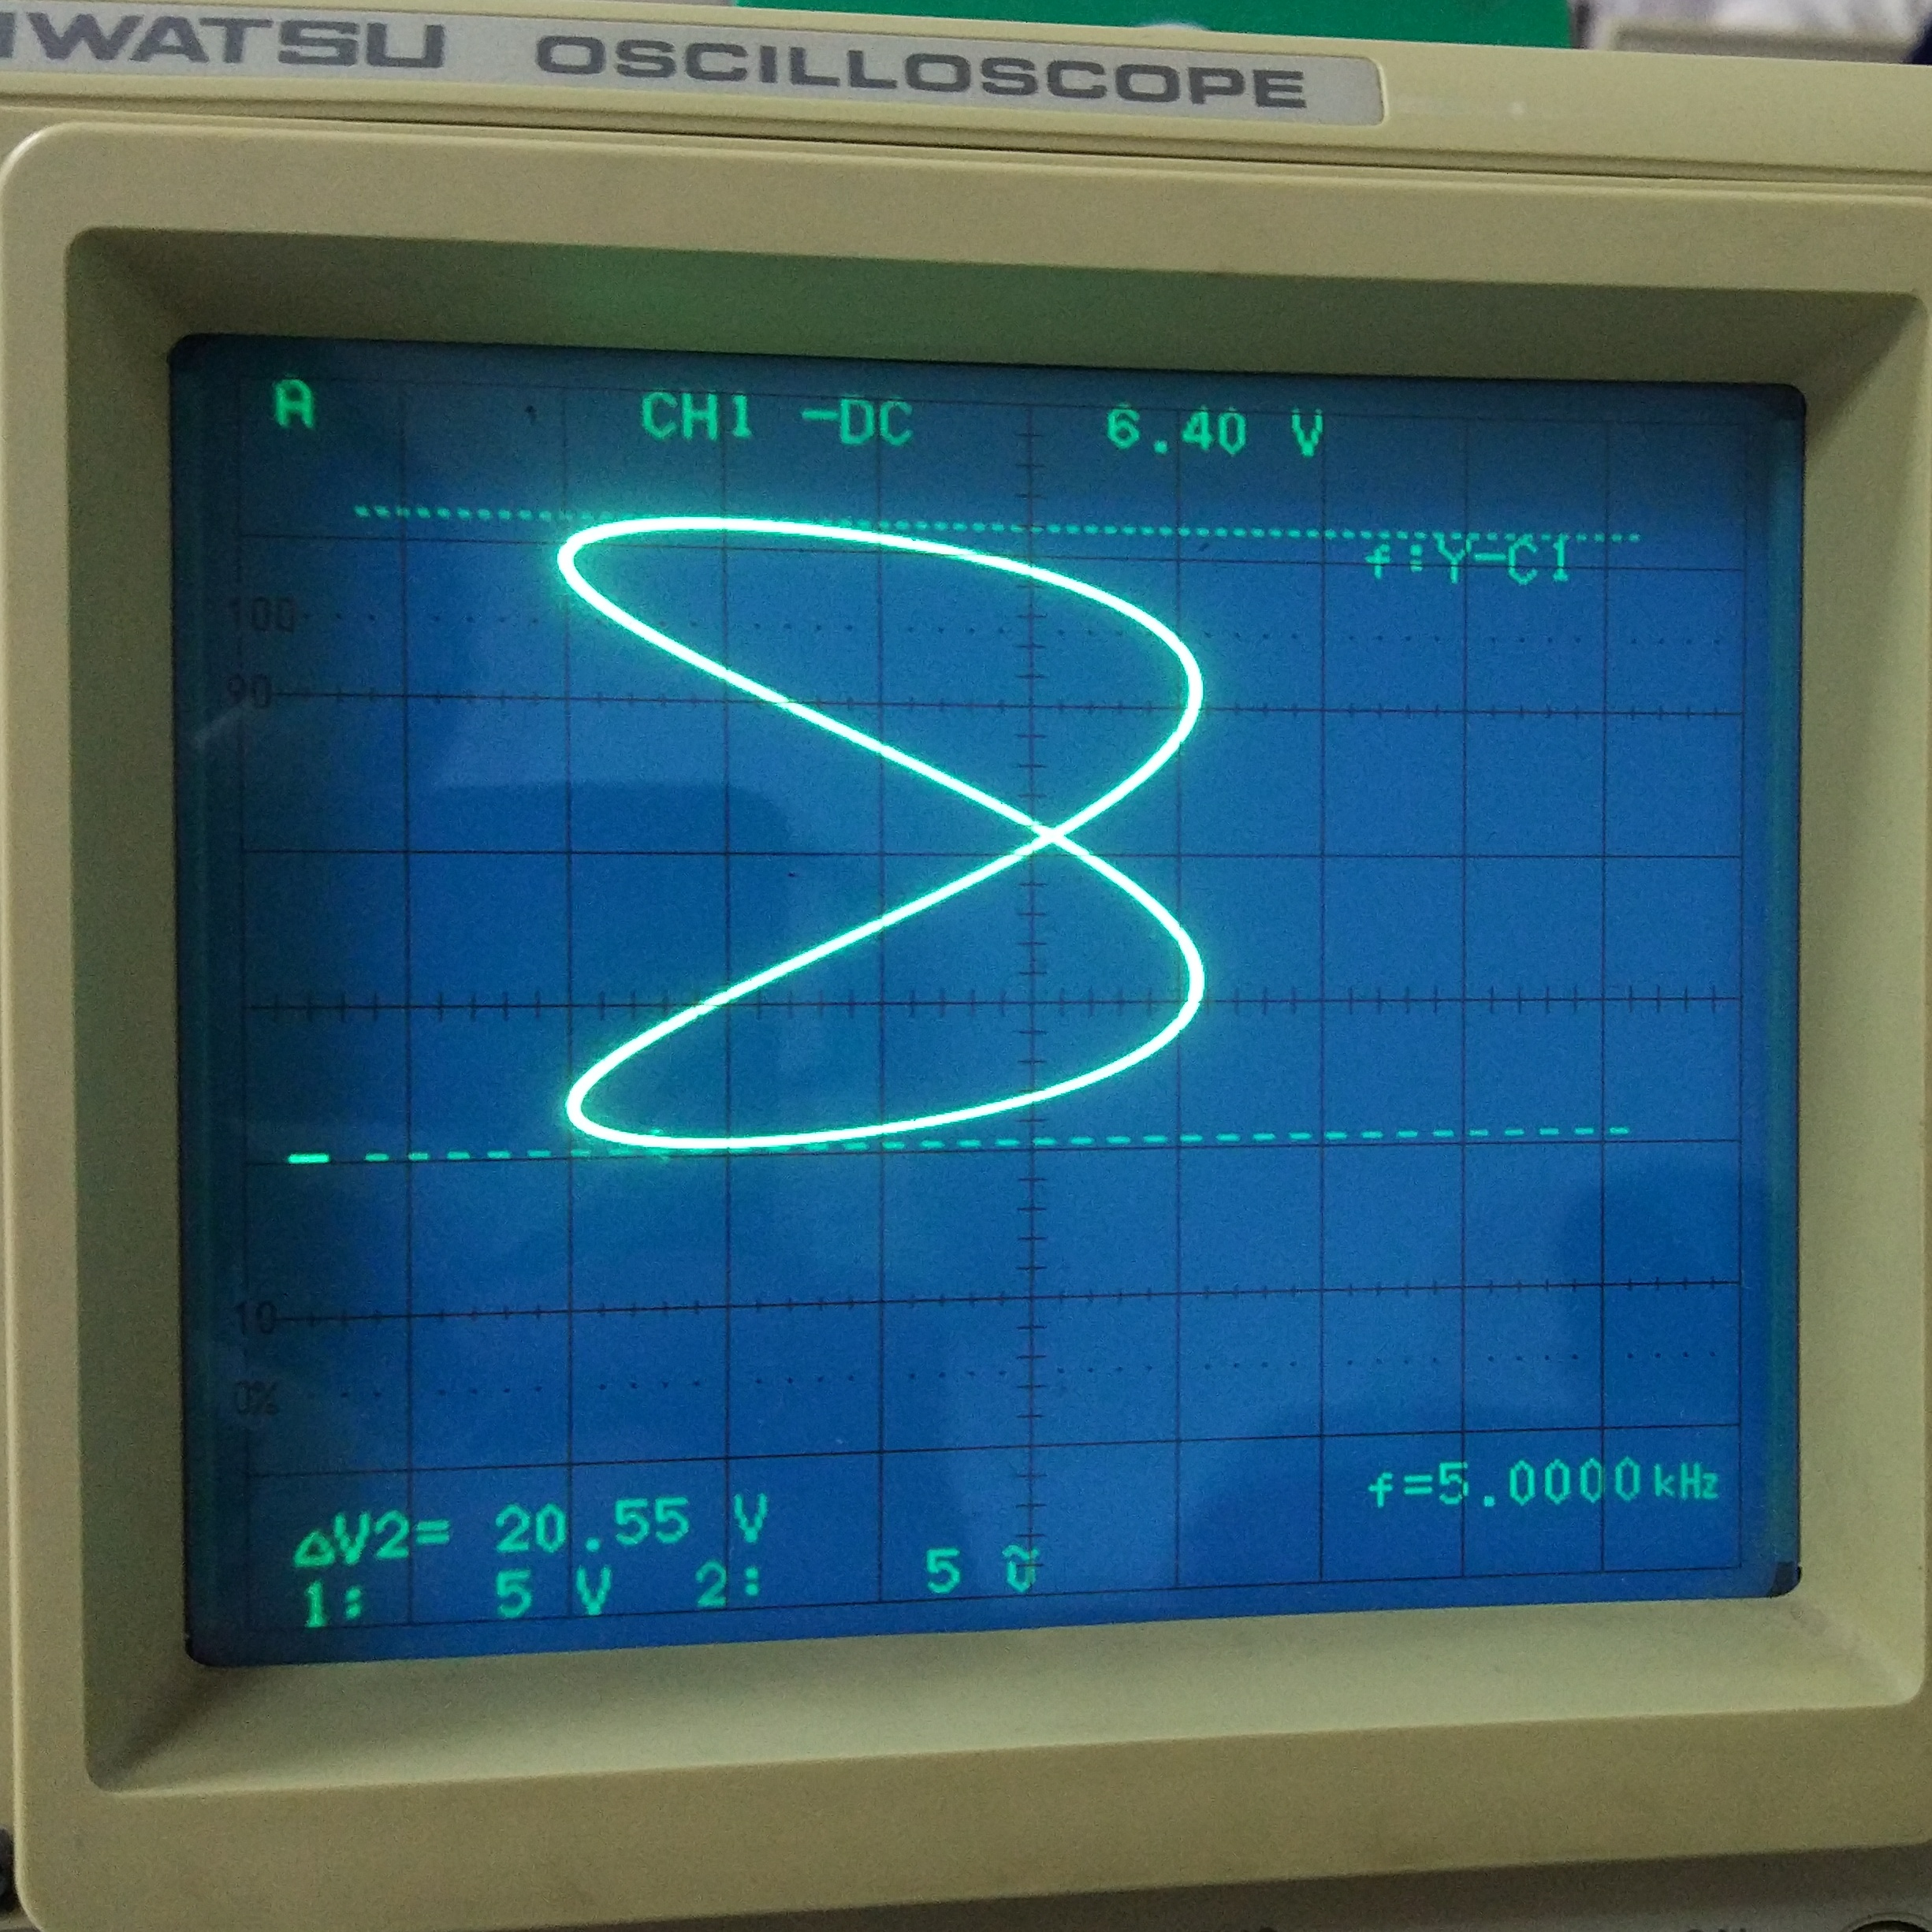
\includegraphics{fig1.jpg}} \\
\subfigure[CH1输入5kHz,CH2输入7.5kHz时的利萨如图形。频率比为2:3。]{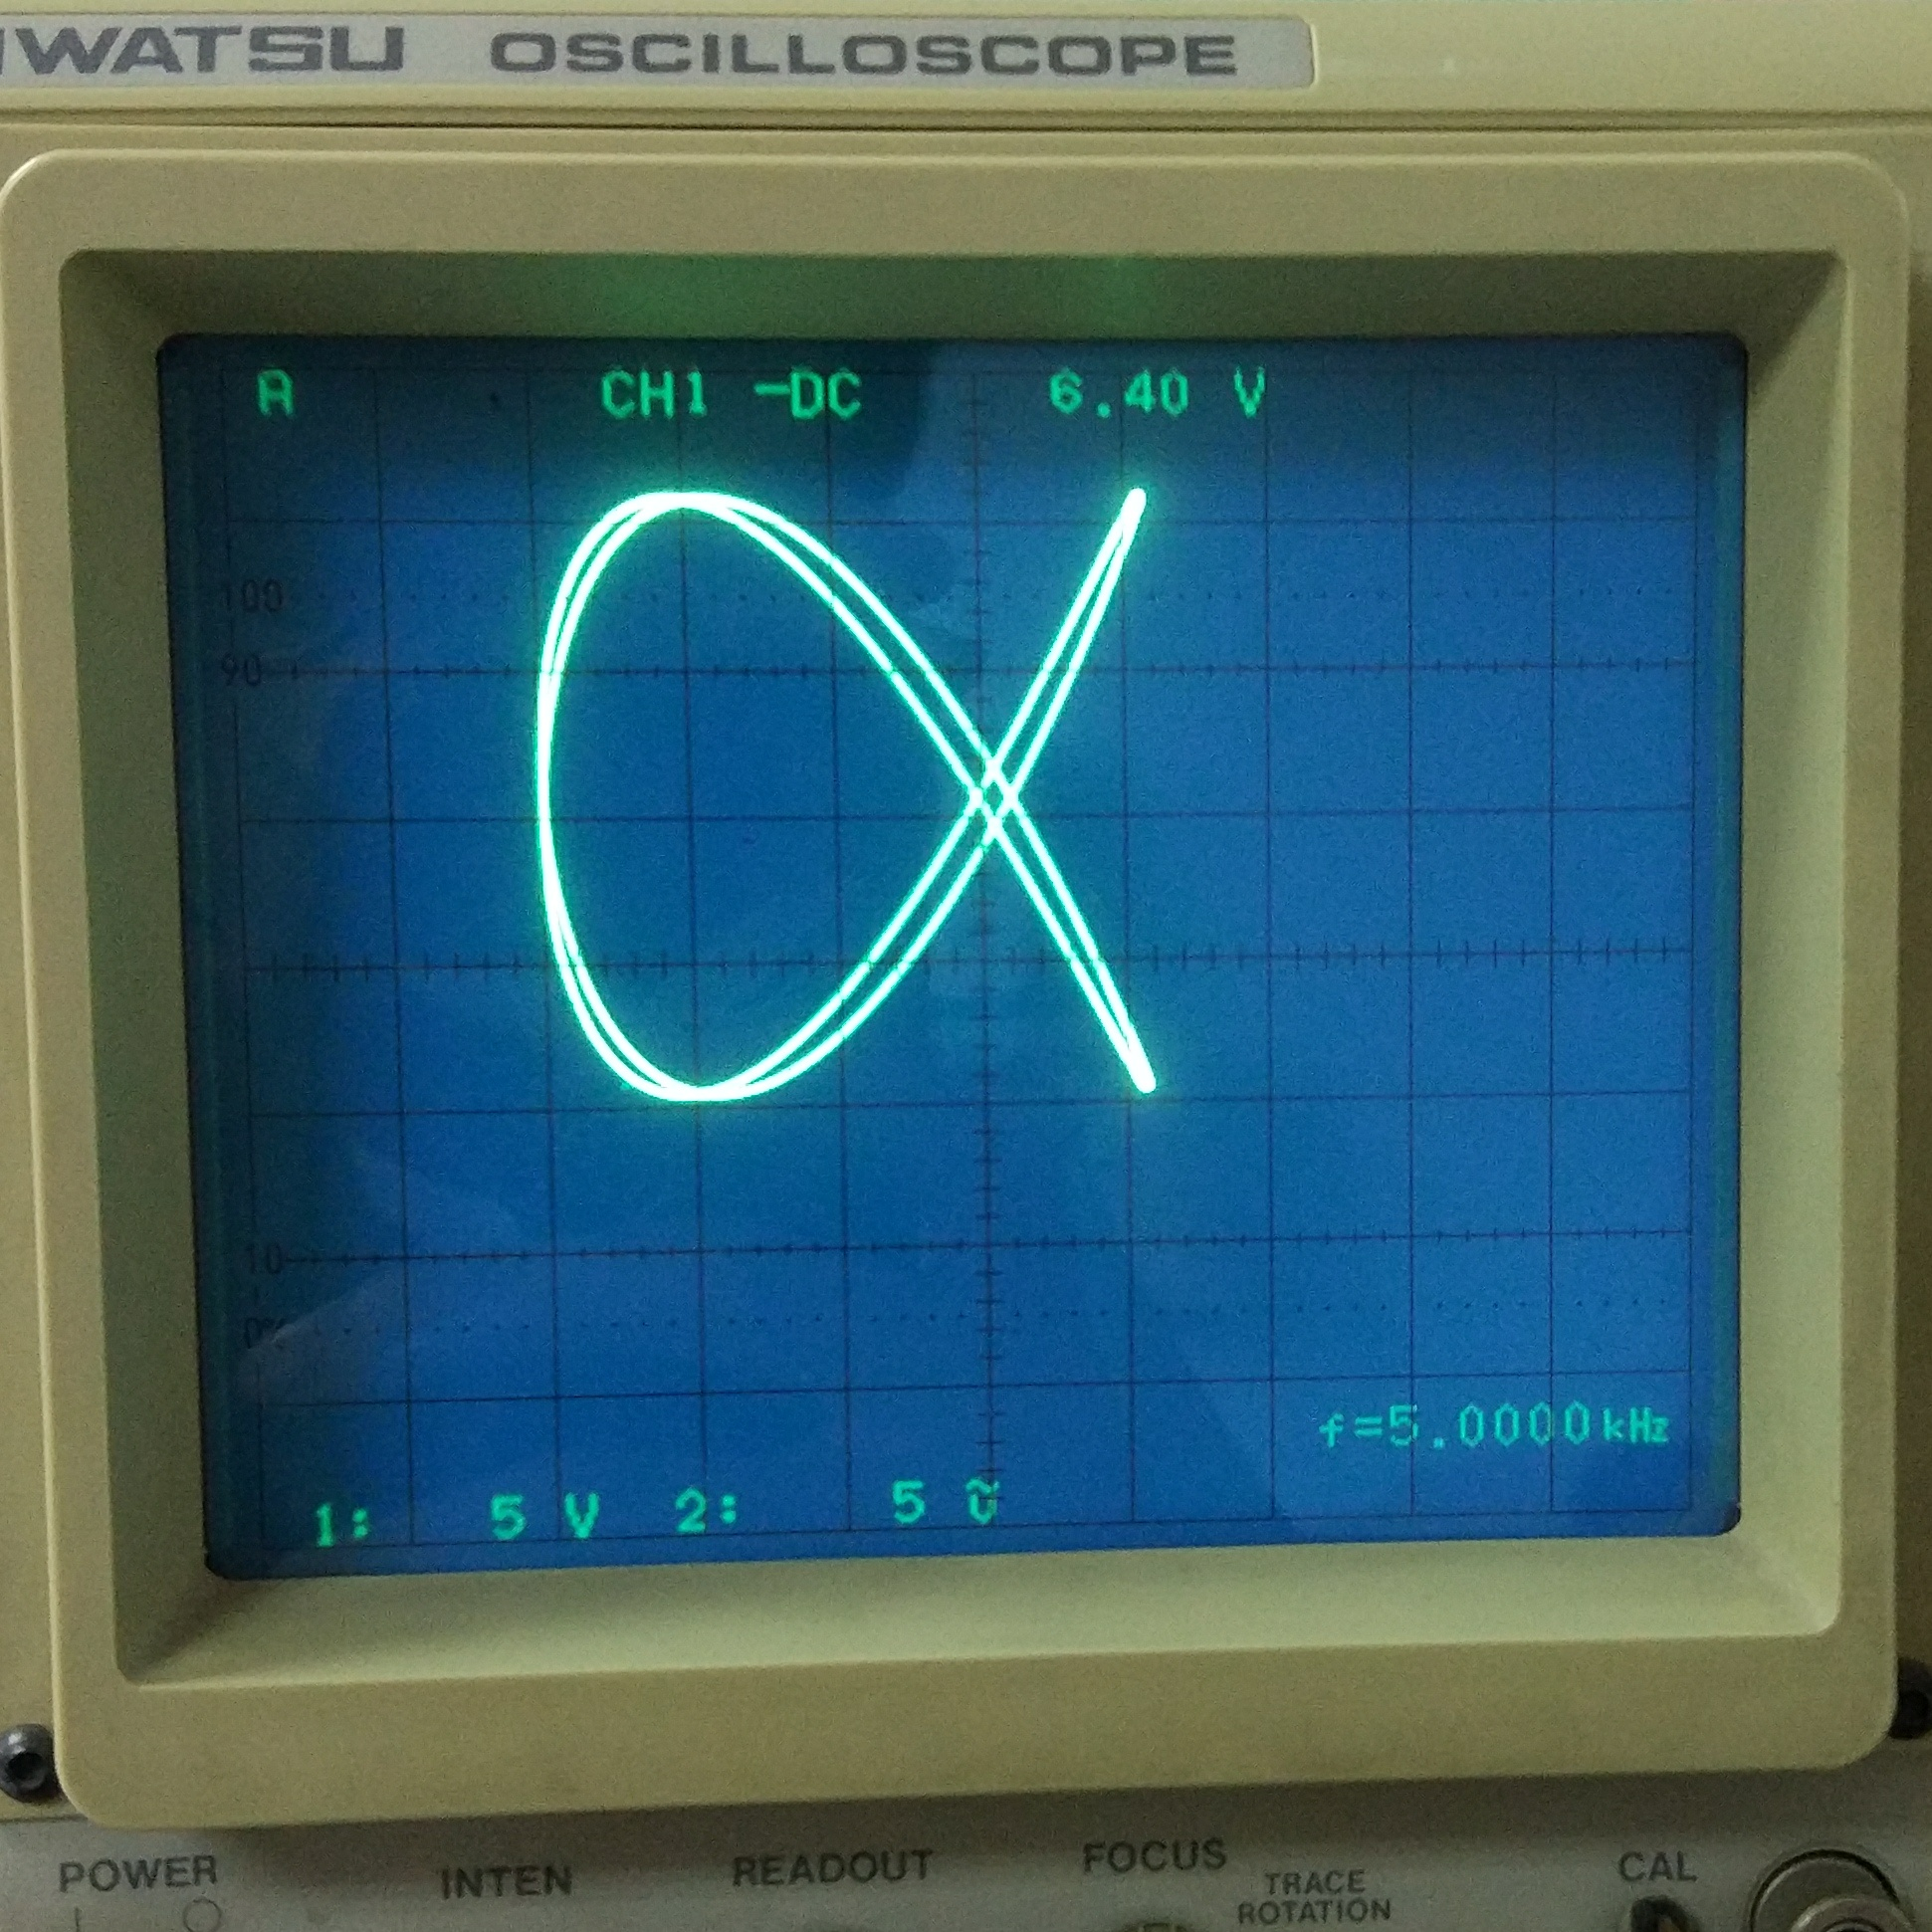
\includegraphics{fig2.jpg}} \\
\subfigure[CH1输入5kHz,CH2输入6kHz时的利萨如图形。频率比为5:6。]{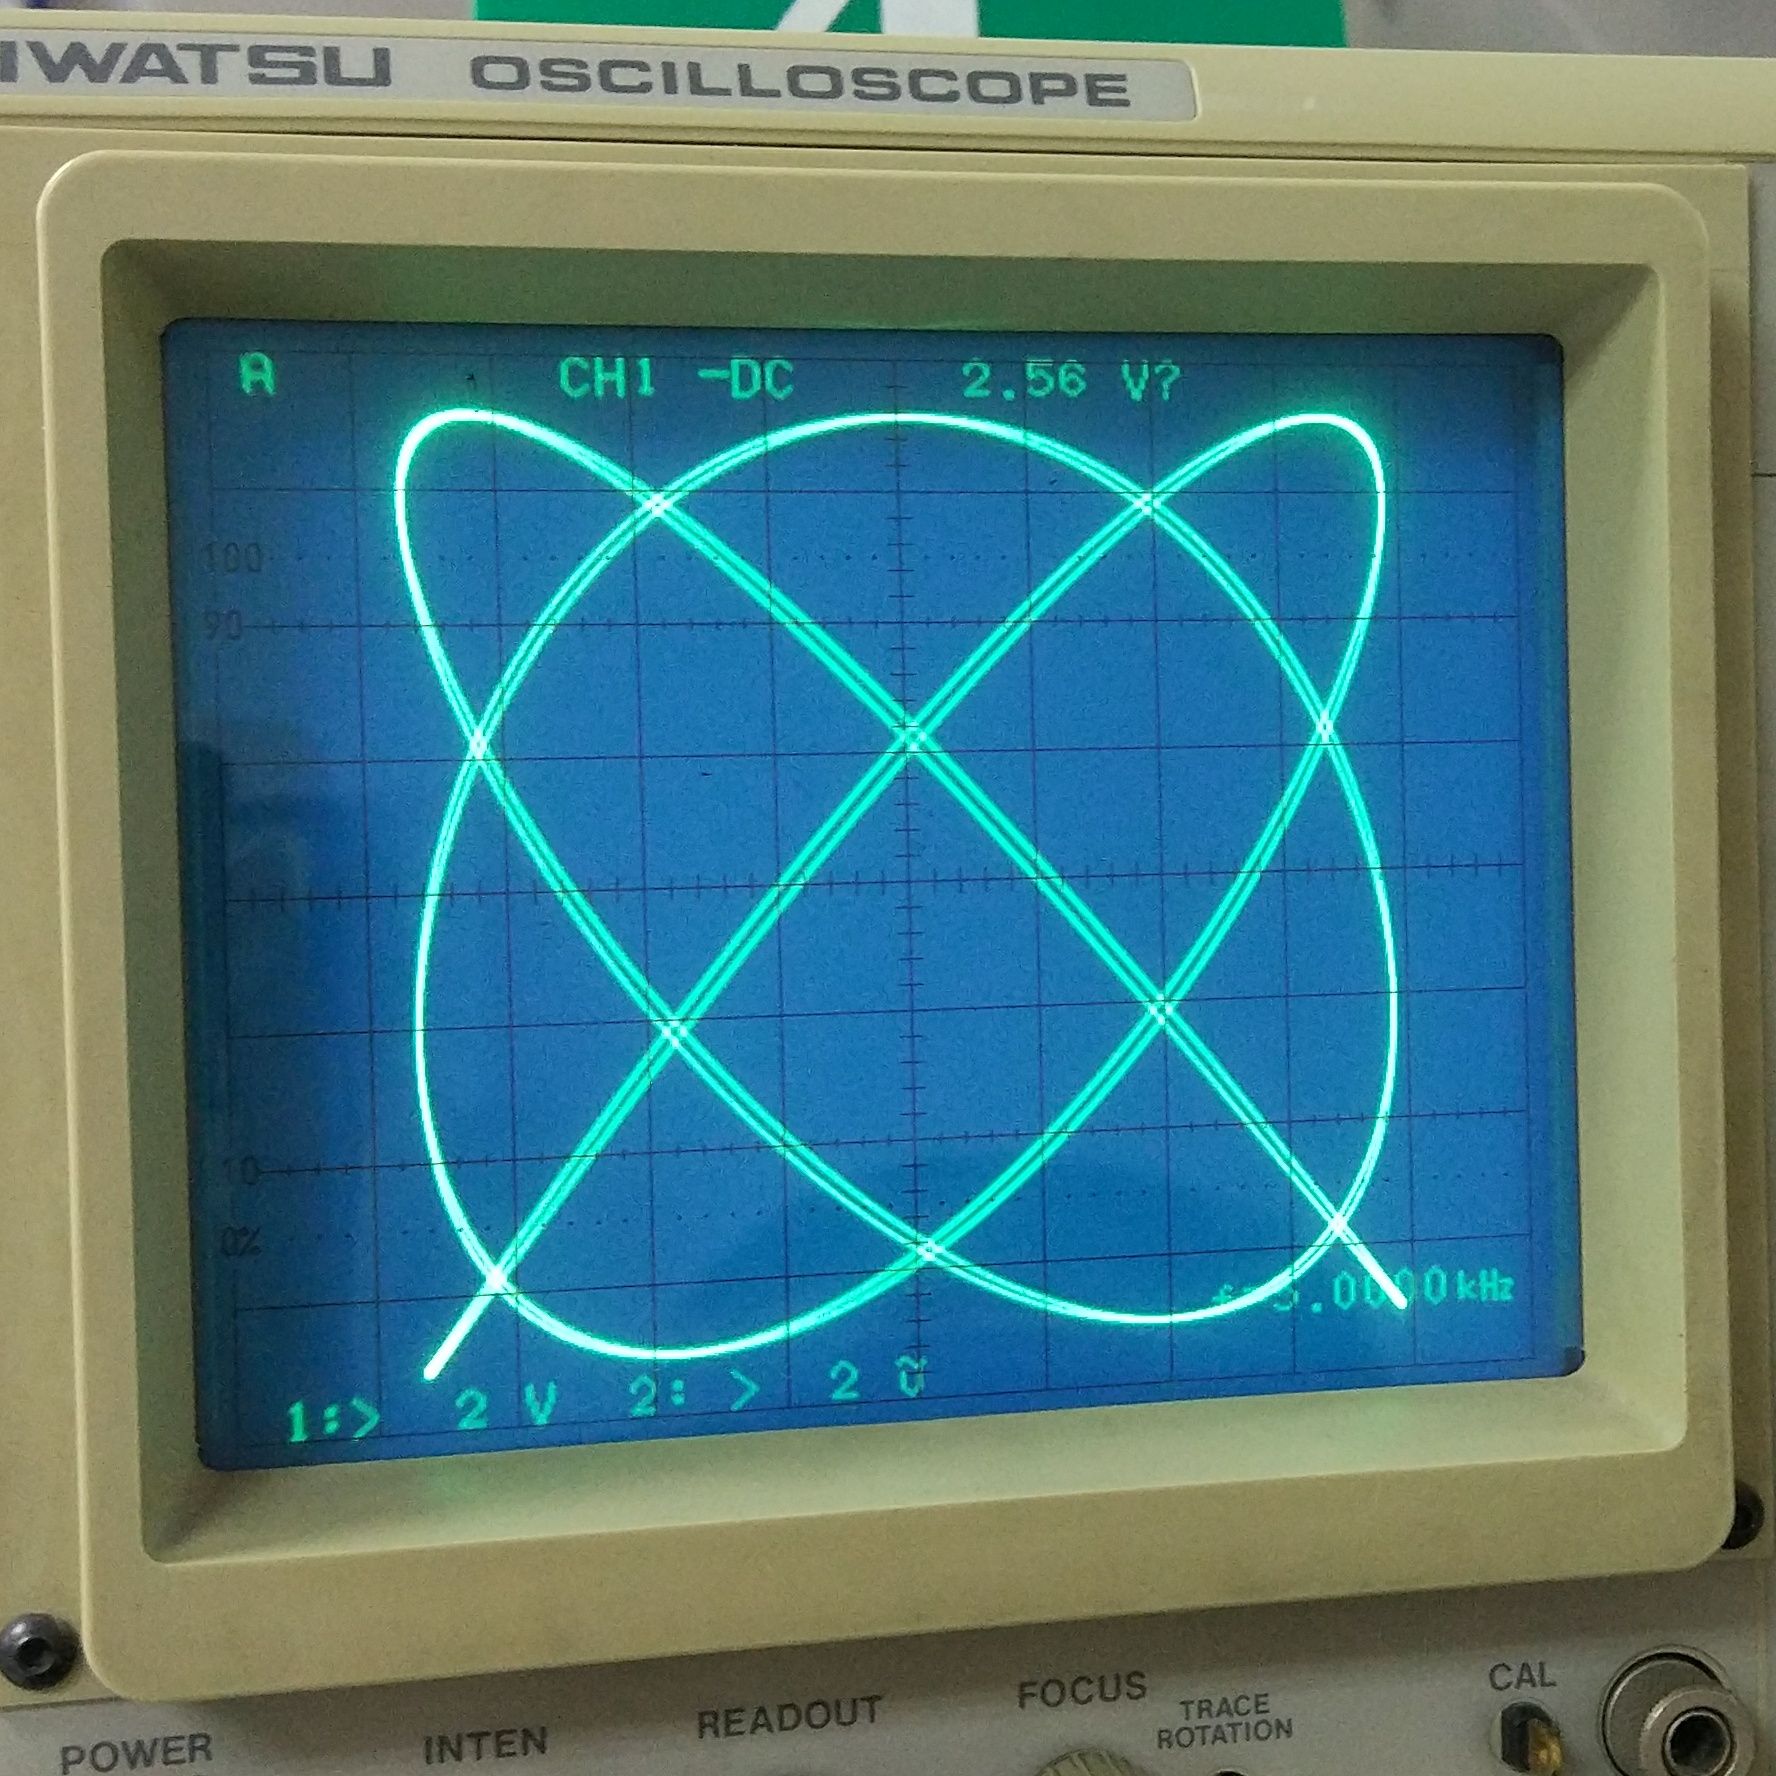
\includegraphics{fig3.jpg}} \\
\caption{将示波器调整至X-Y模式,输入两路频率成简单整数比的信号,在屏幕上观察利萨如图形。}\label{fig:1}
\end{figure}


\end{document}
